\documentclass[pra,12pt]{revtex4}
\usepackage{amsmath}
\usepackage{amssymb}
\usepackage{graphicx}
\usepackage{color}
\usepackage[pdfborder={0 0 0},colorlinks=true,linkcolor=blue,urlcolor=blue]{hyperref}

\def\ket#1{\left|#1\right\rangle}
\def\bra#1{\left\langle#1\right|}
\def\braket#1{\left\langle#1\right\rangle}

\setlength{\parindent}{0pt}

\renewcommand{\baselinestretch}{1.0}
\setlength{\parskip}{0.07in}

\begin{document}

\section*{Appendix B: The Transfer Matrix Method}

The \textbf{transfer matrix method} is a numerical method for solving
the 1D Schr\"odinger equation, and other similar equations.  In this
method, the wavefunction at each point is decomposed into two complex
numbers, called wave components.  The wave components at any two
points are related by a complex $2\times2$ matrix, called the
\textbf{transfer matrix}.

\section{Wave components in 1D}

For a 1D space with spatial coordinates $x$, the Schr\"odinger wave
equation is
$$-\frac{\hbar^2}{2m}\frac{d^2\psi}{dx^2} + V(x) \psi(x) = E\psi(x),$$
where $m$ is the particle mass, $\psi(x)$ is the wavefunction, $V(x)$
is the potential function, and $E$ is the energy.  We treat $E$ as an
adjustable parameter (e.g., the energy of the incident particle in a
scattering experiment).

Within any region of space where $V$ is constant, the Schr\"odinger
equation reduces to a 1D Helmholtz equation, whose general solution is
$$\psi(x) = A\, e^{ik x} + B\, e^{-ik x}, \;\;\; \mathrm{where}\;\; k = \sqrt{\frac{2m[E-V(x)]}{\hbar^2}}.$$
If $E > V$, then the wave-number $k$ is real and positive, and
$\exp(\pm ikx)$ denotes a right-moving ($+$) or left-moving ($-$)
wave.  If $E < V$, then $k$ is purely imaginary, and we choose the
branch of the square root so that it is a positive multiple of $i$, so
that $\exp(\pm ikx)$ denotes a wave that \textit{decreases}
exponentially toward the right ($+$) or toward the left ($-$).

We can re-write the two terms on the right-hand side as
$$\psi(x) = \psi_+(x) + \psi_-(x).$$
At each position $x$, the complex quantities $\psi_\pm(x)$ are called
the \textbf{wave components} .

The problem statement for the transfer matrix method is as follows.
Suppose we have a \textbf{piecewise-constant potential function}
$V(x)$, which takes on values $\{V_1, V_2, V_3, \dots\}$ in different
regions of space, as shown in the figure below:

\begin{center}
  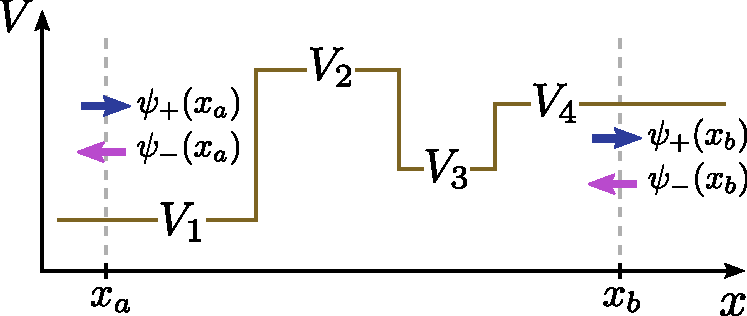
\includegraphics[width=0.45\textwidth]{transfer_matrix_setup}
\end{center}

Given the wave components $\{\psi_+(x_a),\psi_-(x_a)\}$ at one
position $x_a$, we seek to compute the wave components
$\{\psi_+(x_b),\psi_-(x_b)\}$ at another position $x_b$.  In general,
these are related by a linear relation
$$\Psi_b = \mathbf{M}(x_b,x_a) \, \Psi_a,$$
where
$$\Psi_b = \begin{bmatrix}\psi_+(x_b) \\ \psi_-(x_b)\end{bmatrix}, \; \Psi_a = \begin{bmatrix}\psi_+(x_a) \\ \psi_-(x_a)\end{bmatrix}.$$
The $2\times2$ matrix $\mathbf{M}(x_b,x_a)$ is called a
\textbf{transfer matrix}.  Take note of the notation in the
parentheses: we put the ``start point'' $x_a$ in the right-hand input,
and the ``end point'' $x_b$ in the left-hand input.  We want to find
$\mathbf{M}(x_b,x_a)$ from the potential and the energy $E$.

\section{Constructing the transfer matrix}

\subsection{Transfer matrix across a uniform region}

Consider the simplest possible case, where the potential has a single
constant value $V$ everywhere between two positions $x_a$ and $x_b$,
with $x_b > x_a$.  Then, as we have just discussed, the solution
throughout this region takes the form
$$\psi(x) = A e^{ik x} + B e^{-ik x}, \;\;\; \mathrm{where}\;\; k = \sqrt{\frac{2m(E-V)}{\hbar^2}},$$
for some $A, B\in\mathbb{C}$.  The wave components at the two
positions are
$$\Psi_a = \begin{bmatrix} A e^{ik x_a} \\ B e^{ikx_a} \end{bmatrix}, \;\; \Psi_b = \begin{bmatrix} A e^{ik x_b} \\ B e^{ikx_b} \end{bmatrix}.$$
Each component of $\Psi_b$ is $\exp[ik(x_b-x_a)]$ times the
corresponding component of $\Psi_a$.  We can therefore eliminate $A$
and $B$, and write
$$\Psi_b = \mathbf{M}_0(k, x_b-x_a) \Psi_a, \;\;\;\mathrm{where}\;\;\; \mathbf{M}_0(k,L) \equiv \begin{bmatrix}e^{ikL} & 0 \\ 0 & e^{-ikL}\end{bmatrix}.$$
The $2\times2$ matrix $\mathbf{M}_0(k,L)$ is the transfer matrix
across a segment of constant potential.  Its first input is the
wave-number within the segment (determined by the energy $E$ and
potential $V$), and its second input is the segment length.

\subsection{Transfer matrix across a potential step}

Next, consider a potential step occurring at some position $x_0$, as
shown in the figure below:

\begin{center}
  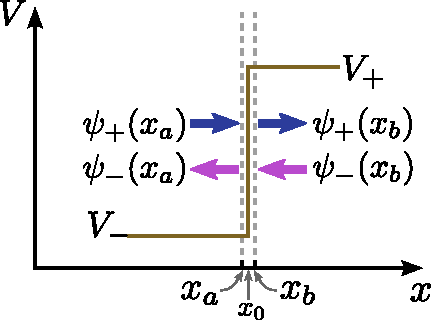
\includegraphics[width=0.32\textwidth]{transfer_step}
\end{center}

Let $x_a$ and $x_b$ be two points that are infinitesimally close to
the potential step on either side (i.e., $x_a = x_0 - 0^+$ and $x_b =
x_0 + 0^+$, where $0^+$ denotes a positive infinitesimal).  To the
left of the step, the potential is $V_-$; to the right, the potential
is $V_+$.  The corresponding wave-numbers are
$$k_\pm = \sqrt{\frac{2m(E-V_\pm)}{\hbar^2}}.$$

There are two important relations between the wavefunctions on the two
sides of the step.  Firstly, any quantum mechanical wavefunction must
be continuous everywhere (otherwise, the Schr\"odinger equation would
not be well-defined); this includes the point $x_0$, so
$$\psi_+(x_a) + \psi_-(x_a) = \psi_+(x_b) + \psi_-(x_b).$$

Secondly, since the potential is non-singular at $x_0$ the derivative
of the wavefunction should be continuous at that point (this can be
shown formally by integrating the Schr\"odinger across an
infinitesimal interval around $x_0$).  Hence,
$$ik_-\, \left[\psi_+(x_a) - \psi_-(x_a)\right] = ik_+\, \left[\psi_+(x_b) - \psi_-(x_b)\right].$$
These two equations can be combined into a single matrix equation:
$$\begin{bmatrix}1 & 1 \\ k_- & - k_-\end{bmatrix}\begin{bmatrix}\psi_+(x_a) \\ \psi_-(x_a) \end{bmatrix} = \begin{bmatrix}1 & 1 \\ k_+ & - k_+\end{bmatrix} \begin{bmatrix}\psi_+(x_b) \\ \psi_-(x_b) \end{bmatrix}.$$
After doing a matrix inversion, this becomes
$$\Psi_b = \mathbf{M}_s(k_+,k_-) \, \Psi_a, \;\;\;\mathrm{where}\;\; \mathbf{M}_s(k_+,k_-) = \frac{1}{2} \begin{bmatrix}1+\frac{k_-}{k_+} & 1-\frac{k_-}{k_+} \\ 1-\frac{k_-}{k_+} & 1+\frac{k_-}{k_+}\end{bmatrix}.$$
The $2\times2$ matrix $\mathbf{M}_s(k_+,k_-)$ is the transfer matrix
to go rightward from a region of wave-number $k_-$, to a region of
wave-number $k_+$.  Note that when $k_- = k_+$, this reduces to the
identity matrix, as expected.

\subsection{Transfer matrix across a piecewise-constant system}

Using the results of the previous two sections, we can find the
transfer matrix for any piecewise-constant potential.  Suppose we have
a potential function which is divided into segments of length $L_1,
L_2, \dots L_N$, with the values $V_1, V_2, \dots, V_N$, as shown
below:

\begin{center}
  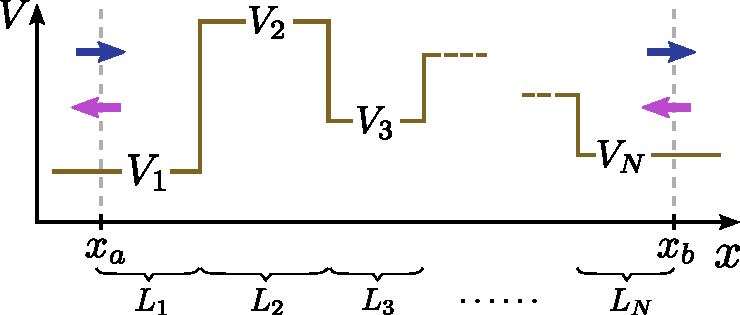
\includegraphics[width=0.5\textwidth]{transfer_matrix_setup2}
\end{center}

Let $x_a$ and $x_b$ lie at the ends of the first and last segments; we
assume that $x_b > x_a$.  We can compute $\Psi_b$ by starting with
$\Psi_a$, and left-multiplying by a sequence of transfer matrices, one
after the other.  These transfer matrices consist of the two types
derived in the previous sections: $\mathbf{M}_0$ (to cross a uniform
segment) and $\mathbf{M}_s$ (to cross a potential step).  Each matrix
multiplication ``transfers'' us to another point to the right, until
we reach $x_b$.

Therefore, the overall transfer matrix between the two points is
$$\boxed{\;\;\;\begin{aligned}\mathbf{M}(x_b, x_a) &= \mathbf{M}_0(k_N,L_N) \; \mathbf{M}_s(k_N, k_{N-1}) \cdots \mathbf{M}_0(k_2,L_2) \; \mathbf{M}_s(k_2, k_1) \; \mathbf{M}_0(k_1,L_1) \;\;\;\\ \mathrm{where}\;\;\; \mathbf{M}_0(k,L) &= \begin{bmatrix}e^{ikL} & 0 \\ 0 & e^{-ikL}\end{bmatrix} \\ \mathbf{M}_s(k_+,k_-) &= \frac{1}{2} \begin{bmatrix}1+\frac{k_-}{k_+} & 1-\frac{k_-}{k_+} \\ 1-\frac{k_-}{k_+} & 1+\frac{k_-}{k_+}\end{bmatrix}\\ k_n &= \sqrt{\frac{2m(E-V_n)}{\hbar^2}}.\end{aligned}}$$
The expression for $\mathbf{M}(x_b,x_a)$ should be read from right to
left.  Starting from $x_a$, we cross segment 1, then cross the
potential step from segment 1 to segment 2, then cross segment 2, and
so forth.  (A common mistake, when writing transfer matrix code, is to
assemble the matrices left-to-right, i.e.~right-multiplying when you
should be left-multiplying.)



\end{document}


== Wave scattering in 1D ==

The transfer matrix method is typically used to study how a structure, such as a block of dense material, scatters an incident wave (be it an electromagnetic wave, a sound wave, or any other kind of wave describable by the 1D wave equation).  Let us consider a finite structure suspended in empty space.  For positions $x$ lying in some finite region, the refractive index function $n(x)$ varies in a particular way, but the rest of space is empty, so

: $n(x) = 1 \quad \mathrm{for}\;\mathrm{large}\;\, |x|.$

We are interested in what happens when a wave is incident on the structure from the empty-space region.  For the moment, let's suppose the incident wave is coming from the left.  The wave will be scattered as it meets the structure, and in 1D (but not in higher dimensions), the scattering consists of two distinct processes: part of the wave will be ''reflected'' back to the left, while another part will be ''transmitted'' across the structure and into the empty-space region on the right.

This can be described in terms of wave components.  If we pick an arbitrary point $x_a$ in the empty-space region on the left, the right-moving wave component $\psi_+(x_a)$ corresponds to the incident wave, and the left-moving wave component $\psi_-(x_a)$ corresponds to reflected wave.  Picking an arbitrary point $x_b$ in the empty-space region on the right, the right-moving wave component $\psi_+(x_b)$ corresponds to the transmitted wave, and ''the left-moving wave component is zero'' since there is (by assumption) no wave incident from the right.

==== Reflection and transmission coefficients ====

We define the "reflection coefficient" $r$ as the ratio of the reflected to incident wave components, and the "transmission coefficient" $t$  as the ratio of the transmitted to incident wave components:

: $r = \frac{\psi_-(x_a)}{\psi_+(x_a)},\quad t = \frac{\psi_+(x_b)}{\psi_+(x_a)}.$

Note that both $r$ and $t$ are complex numbers.  Now, using the fact that the wave components are related by the transfer matrix equation

:$\mathbf{M}(x_b,x_a) \begin{bmatrix}\psi_+(x_a) \\ \psi_-(x_a)\end{bmatrix} = \begin{bmatrix}\psi_+(x_b) \\ 0\end{bmatrix},$

one can easily show that

: $r = \frac{M_{21}}{M_{22}}, \quad t = \frac{M_{11} M_{22} - M_{12}M_{21}}{M_{22}}.$

Here, $M_{ij}$ denotes the $i,j$ matrix element of $\mathbf{M}(x_b,x_a)$.  The reflection and transmission coefficients depend on the transfer matrix (and hence on the refractive index function and the frequency).  They do ''not'' depend on the magnitude of the incident wave.  This is to be expected, because of the linearity of the wave equation: if we change the amplitude of the incident wave, the reflected and transmitted waves change by a proportionate factor, which leaves $r$ and $t$ unaffected due to their definition as ratios.

==== Reflectance and transmittance ====

The squared magnitude of the reflection coefficient, $R \equiv |r|^2$, is called the "reflectance".  The squared magnitude of the transmission coefficient, $T \equiv |t|^2$, is called the "transmittance".  When $n(x)$ is everywhere real, the reflectance and transmittance obey the equation

: $R + T = 1.$

The squared amplitude of a traveling wave can be interpreted as its "intensity": a quantity that describes the rate at which energy is transported along by the wave.  Thus, $R$ and $T$ correspond to the intensities of the reflected and transmitted waves, normalized to the intensity of the incident wave.  The fact that they sum up to one is thus a statement of the conservation of energy.

The conservation equation can be derived from the wave equation.  [[Energy conservation in 1D wave equation|See this page for the proof.]]

==== Example: scattering from a uniform block ====

As a simple but instructive example of wave scattering, consider a uniform block of refractive index $n_1$ and length $L$.  The refractive index function is

: $n(x) = \left\{\begin{array}{ll}n_1, & 0 \le x \le L,\\ 1 & \mathrm{otherwise}. \end{array}\right.$

In the context of wave scattering, this kind of uniform block structure is called an "etalon", a French word meaning "standard” (because it is the simplest example of a non-trivial scatterer).

It suffices to place the measurement points $x_a$ and $x_b$ infinitesimally to the left and right of the etalon, respectively.  Then, according to the formula we have developed [[#Transfer matrix across a piecewise-constant system|above]], the transfer matrix is

: $\mathbf{M} = \mathbf{Q}(1,n_1)\,\mathbf{P}(n_1,L)\,\mathbf{Q}(n_1,1).$

The transfer matrix also depends on the frequency $\omega$, which enters in the sub-matrix $\mathbf{P}$.  Further examination reveals that the etalon's transfer matrix has a special property: it depends on $\omega$ and $L$ only via the combination $\omega L$.

We can compute the transfer matrix numerically, and hence obtain the reflectance and transmittance.  The results are shown in Fig. 4.  The reflectance and transmittance are plotted against $\omega L$, which we could either think of as varying $L$ while keeping $\omega$ fixed, or vice versa.  Also plotted are the complex arguments of the reflection and transmission coefficients.  These quantities are physically meaningful too; they reveal how the phase of the reflected or transmitted wave changes as we vary the scatterer length $L$, keeping the wave frequency $\omega$ fixed.

[[File:Etalon rt.svg|frame|center|upright|Fig. 4: Reflectance and transmittance (upper plots), and the complex arguments of the reflection and transmission coefficients (lower plots), versus $\omega L$, for uniform blocks of refractive index $n_1=3$ and $n_1=10$.]]

The scattering behavior of the etalon exhibits several interesting features:

* For $\omega L \rightarrow 0$, the wave is completely transmitted, with zero reflection.  Thus, an etalon is ineffective at scattering a wave whose wavelength is much larger than itself.
* Apart from $\omega L = 0$ limit, there are certain multiples of $\omega L$ where the transmittance goes to unity and the reflectance goes to zero.  These are called "transmission resonances", and with a bit more work it's possible to show that they occur when<br/>&nbsp;&nbsp;&nbsp;$n_1 \omega L = m\pi,\quad m \in \mathbb{Z}^+.$<br/>Since the wavelength inside the etalon medium is $2\pi/n_1 \omega$, transmission resonances occur when a half-integer or integer number of wavelengths fit exactly inside the etalon.  This phenomenon is thus an outcome of wave interference.
* During each resonance "cycle", the phases of both the reflected and transmitted waves advance by $\pi$.
* For larger values of $n_1$, it can be shown that the transmission resonances become narrower.  Thus, for the $n_1 = 10$ case shown in Fig. 4, the transmission peaks, reflectance dips, and phase advances occur over relatively narrower intervals of $\omega L$.
* For real and positive $n_1$, there is no "reflection resonance" phenomenon in which the reflectance goes to unity.  Some of the wave always makes it through the etalon.

Many of these features are also present when looking at wave scattering in higher dimensions, and for more complicated structures.  We will revisit the physics of wave scattering later, after learning a bit more mathematical technology such as [[Green's function|the Green's function method]].

== Exercises ==

<ol>
<li>
By modifying [[Energy conservation in 1D wave equation|our earlier proof]] that $R + T = 1$ for real refractive index, show that $R + T \le 1$ if $\mathrm{Im}[n(x)] \ge 1$.</li>
<li>The conservation relation $R + T = 1$ was derived by assuming that the two regions on the far left and far right have equal refractive index (i.e., the scatterer is suspended in a uniform medium, such as vacuum).  Now suppose the two regions on the far left and far right have different refractive index: let $n(x) = n_a$ on the far left, and $n(x) = n_b$ on the far right, where $n_a, n_b \in \mathbb{R}$.  Derive a generalization of the conservation relation.</li>
<li>Consider a structure consisting of $N$ layers of uniform refractive index $n_1 = 1.05$ and equal length $L = 1$, separated from one another by gaps of uniform refractive index 1 and length $L = 1$.  The rest of space is empty, with refractive index $ n = 1$.
<ol style="list-style-type:lower-alpha">
<li>Write a program to compute, via the transfer matrix, the reflectance $R$ and transmittance $T$ as a function of the frequency $\omega$.  Show the results for $N = 5, 10, 50$.  When the number of layers is large, you should find that the reflectance approaches unity at a certain frequency.  Such a structure is called a ''Bragg reflector''.</li>
<li>By varying $L$ in your program, deduce an approximate expression for the frequency at which the reflectance peak occurs.</li>
<li>For comparison, compute  the $R$ versus $T$ versus $\omega$ plot for a uniform block of refractive index $n_1$ and the same total length.</li>
</ol>
</li>
</ol>


\end{document}

